\documentclass[11pt,a4paper]{article}

\usepackage{fontspec}
\setmainfont{Arial}
\setsansfont{Arial}
\usepackage{amsmath,amssymb}
\usepackage{geometry}
\usepackage{graphicx}
\usepackage{booktabs}
\usepackage{array}
\usepackage{tabularx}
\usepackage{longtable}
\usepackage{caption}
\usepackage{subcaption}
\usepackage{xcolor}
\usepackage{hyperref}
\usepackage[numbers,sort&compress]{natbib}
\usepackage{microtype}

\geometry{margin=24mm}
\hypersetup{
  colorlinks=true,
  linkcolor=blue!55!black,
  citecolor=blue!55!black,
  urlcolor=blue!55!black
}
\setlength{\parskip}{0.55em}
\setlength{\parindent}{0pt}
\sloppy

\newcommand{\R}{\mathbb{R}}
\newcommand{\Y}{\mathcal{Y}}
\newcommand{\X}{\mathcal{X}}
\newcommand{\argmax}{\operatorname*{arg\,max}}
\newcommand{\argmin}{\operatorname*{arg\,min}}
\newcommand{\norm}[1]{\left\lVert #1 \right\rVert}

\title{\textbf{Structural SVM OCR: mathematical setup and fair DBCFW vs DFW comparison}}
\author{Decentralized Block-Coordinate Frank-Wolfe experiments}
\date{June 22, 2026}

\begin{document}
\maketitle

\begin{abstract}
This note documents the Structural SVM OCR experiment used in the repository. We formalize the sequence prediction objective, the loss-augmented Viterbi oracle, the primal and dual Structural SVM formulations, and the Frank-Wolfe family of solvers. The main empirical comparison is not central FW against decentralized DFW. Instead, the fair comparison is decentralized DBCFW against decentralized DFW under the same OCR split, same network setup, same regularization, and a common cost axis: the number of training loss-augmented Viterbi oracle calls. Under this accounting, DBCFW with one block per agent reaches 18.24\% OCR test error using 3,780 training oracle calls, while the nearest DFW point uses 6,251 calls and has 72.20\% test error. Central BCFW is reported only as a sanity reference and reaches 10.95\% best test error.
\end{abstract}

\section{Problem and data}

We consider sequence labeling for the Taskar OCR data used in max-margin structured prediction literature \citep{taskar2003maxmargin,lacostejulien2013bcfw}. Each example is a word image that has already been segmented into characters. The input is a sequence
\[
  x_i = (x_{i1},\ldots,x_{iT_i}), \qquad x_{it}\in\R^{129},
\]
where the 128 pixel features are augmented with a constant bias coordinate. The output is a label sequence
\[
  y_i = (y_{i1},\ldots,y_{iT_i}), \qquad y_{it}\in\{1,\ldots,26\}.
\]
We use the \texttt{ocr2} split: train folds not equal to zero and test fold zero. In the local run this gives 6,251 train words and 626 test words. The total number of train letters is 47,535 and the total number of test letters is 4,617.

The structured feature map decomposes into emission, boundary, and transition features:
\[
  \Phi(x,y) =
  \left[
    \sum_{t=1}^{T} x_t \otimes e_{y_t},
    e_{y_1},
    e_{y_T},
    \sum_{t=2}^{T} e_{y_{t-1}}\otimes e_{y_t}
  \right].
\]
With 129 input features, 26 labels, two boundary-label blocks, and a \(26\times26\) transition table, the dimension is
\[
  d = 129\cdot 26 + 2\cdot 26 + 26^2 = 4082.
\]
Prediction is
\[
  h_w(x) = \argmax_{y\in\Y(x)} \langle w,\Phi(x,y)\rangle .
\]
The evaluation loss is normalized Hamming loss,
\[
  \Delta(y,\hat y) = \frac{1}{T}\sum_{t=1}^{T}\mathbf{1}\{y_t\neq \hat y_t\}.
\]

\section{Structural SVM objective}

We use the margin-rescaled Structural SVM formulation \citep{tsochantaridis2005large,joachims2009cutting}. Define the difference feature vector
\[
  \psi_i(y) = \Phi(x_i,y_i)-\Phi(x_i,y).
\]
The structured hinge for example \(i\) is
\[
  H_i(w) = \max_{y\in\Y(x_i)}
    \left\{
      \Delta(y_i,y) - \langle w,\psi_i(y)\rangle
    \right\}.
\]
The primal objective is
\[
  P(w) =
  \frac{\lambda}{2}\norm{w}^2 +
  \frac{1}{n}\sum_{i=1}^{n} H_i(w).
\]
The loss-augmented inference problem is
\[
  \hat y_i(w) =
  \argmax_{y\in\Y(x_i)}
    \left\{
      \Delta(y_i,y) + \langle w,\Phi(x_i,y)\rangle
    \right\}.
\]
For sequence models with first-order transitions this is solved exactly by Viterbi dynamic programming. In this experiment, one such loss-augmented Viterbi call is the atomic expensive oracle.

The dual used by Frank-Wolfe has one simplex block per training example:
\[
  \alpha_i \in \Delta_{\Y_i}, \qquad i=1,\ldots,n.
\]
Let
\[
  w(\alpha) =
  \frac{1}{\lambda n}
  \sum_{i=1}^{n}\sum_{y\in\Y_i}\alpha_i(y)\psi_i(y),
  \qquad
  \ell(\alpha) =
  \frac{1}{n}
  \sum_{i=1}^{n}\sum_{y\in\Y_i}\alpha_i(y)\Delta(y_i,y).
\]
Then the concave dual objective is
\[
  D(\alpha) =
  \ell(\alpha) -
  \frac{\lambda}{2}\norm{w(\alpha)}^2.
\]
The Frank-Wolfe duality gap can be computed through the same loss-augmented inference oracles, which is one of the practical advantages emphasized by BCFW for Structural SVMs \citep{lacostejulien2013bcfw}.

\section{Classical approaches}

\paragraph{Cutting-plane Structural SVM.}
Classical Structural SVM training solves a quadratic program with exponentially many margin constraints by iteratively adding violated constraints \citep{tsochantaridis2005large,joachims2009cutting}. The method is conceptually clean and strong for batch training, but each iteration requires inference across many or all examples.

\paragraph{Full Frank-Wolfe.}
The original Frank-Wolfe or conditional-gradient method \citep{frank1956algorithm,jaggi2013frankwolfe} is projection-free and only needs a linear minimization oracle. For the Structural SVM dual, a full FW step runs loss-augmented inference for every training block, forms a full search vertex, and then performs a convex update.

\paragraph{Block-coordinate Frank-Wolfe.}
BCFW updates one example block, or a mini-batch of blocks, at a time. Lacoste-Julien et al. show that this is particularly natural for Structural SVMs because the dual feasible set is a Cartesian product of simplices and the block oracle is just one loss-augmented inference problem \citep{lacostejulien2013bcfw}. This lowers the per-iteration cost while preserving useful duality-gap certificates.

\paragraph{Decentralized Frank-Wolfe.}
Decentralized FW methods combine conditional-gradient steps with network averaging or consensus over agents \citep{wai2017decentralized}. Our experiment follows this projection-free decentralized viewpoint. Agents own disjoint parts of the OCR training set and communicate through an Erdos-Renyi graph.

\section{What we compare}

The main comparison is decentralized DBCFW vs decentralized DFW on the same OCR Structural SVM task. It is important not to confuse the following two comparisons.

\begin{enumerate}
  \item \textbf{Decentralized DBCFW vs DFW.} This is the main result. Both methods use the same train/test split, same regularization \(\lambda=1/n\), same 7-agent partition, same graph seed, and same decentralized communication model. They differ in block budget. DBCFW uses \(B=1\), while DFW uses the full local block budget \(B=893\).
  \item \textbf{Central BCFW vs FW.} This is a sanity/reference validation of the Structural SVM implementation against the paper-style central setup. It is not used as the DFW baseline.
\end{enumerate}

The cost axis is \emph{training oracle calls}. A training oracle call is one loss-augmented Viterbi call used by an update. Diagnostic calls used only to evaluate test error or full duality gap are excluded from the cost axis.

For the decentralized OCR run:
\[
  \text{cost per DBCFW iteration with }B=1 = 7\cdot 1 = 7,
\]
while
\[
  \text{cost per DFW iteration with }B=893 = 7\cdot 893 = 6251.
\]
Therefore, comparing raw iteration counts would be misleading. DBCFW can perform many cheap block updates before DFW completes one full local update. The fair question is: for a comparable number of loss-augmented Viterbi oracle calls, which method obtains lower test error?

\section{Experimental setup}

The local artifacts used in this report are:
\begin{itemize}
  \item \path{runs_paper_ocr/ocr_decentralized_fair_oracle_extra/results.csv}: main fair DBCFW vs DFW sweep.
  \item \path{runs_paper_ocr/ocr_full_140_passes/results.csv}: central BCFW/FW sanity reference.
\end{itemize}
The decentralized fair sweep used:
\[
  N=7,\quad K=893,\quad \lambda\in\{0.01,0.001,1/n\}.
\]
For DFW we used the full block \(B=893\) and logged the first 25 iterations densely. For DBCFW we ran \(B=1\) for 900 iterations, \(B=10\) for 200 iterations, and \(B=89\) for 160 iterations.

\section{Main result}

\begin{figure}[htbp]
  \centering
  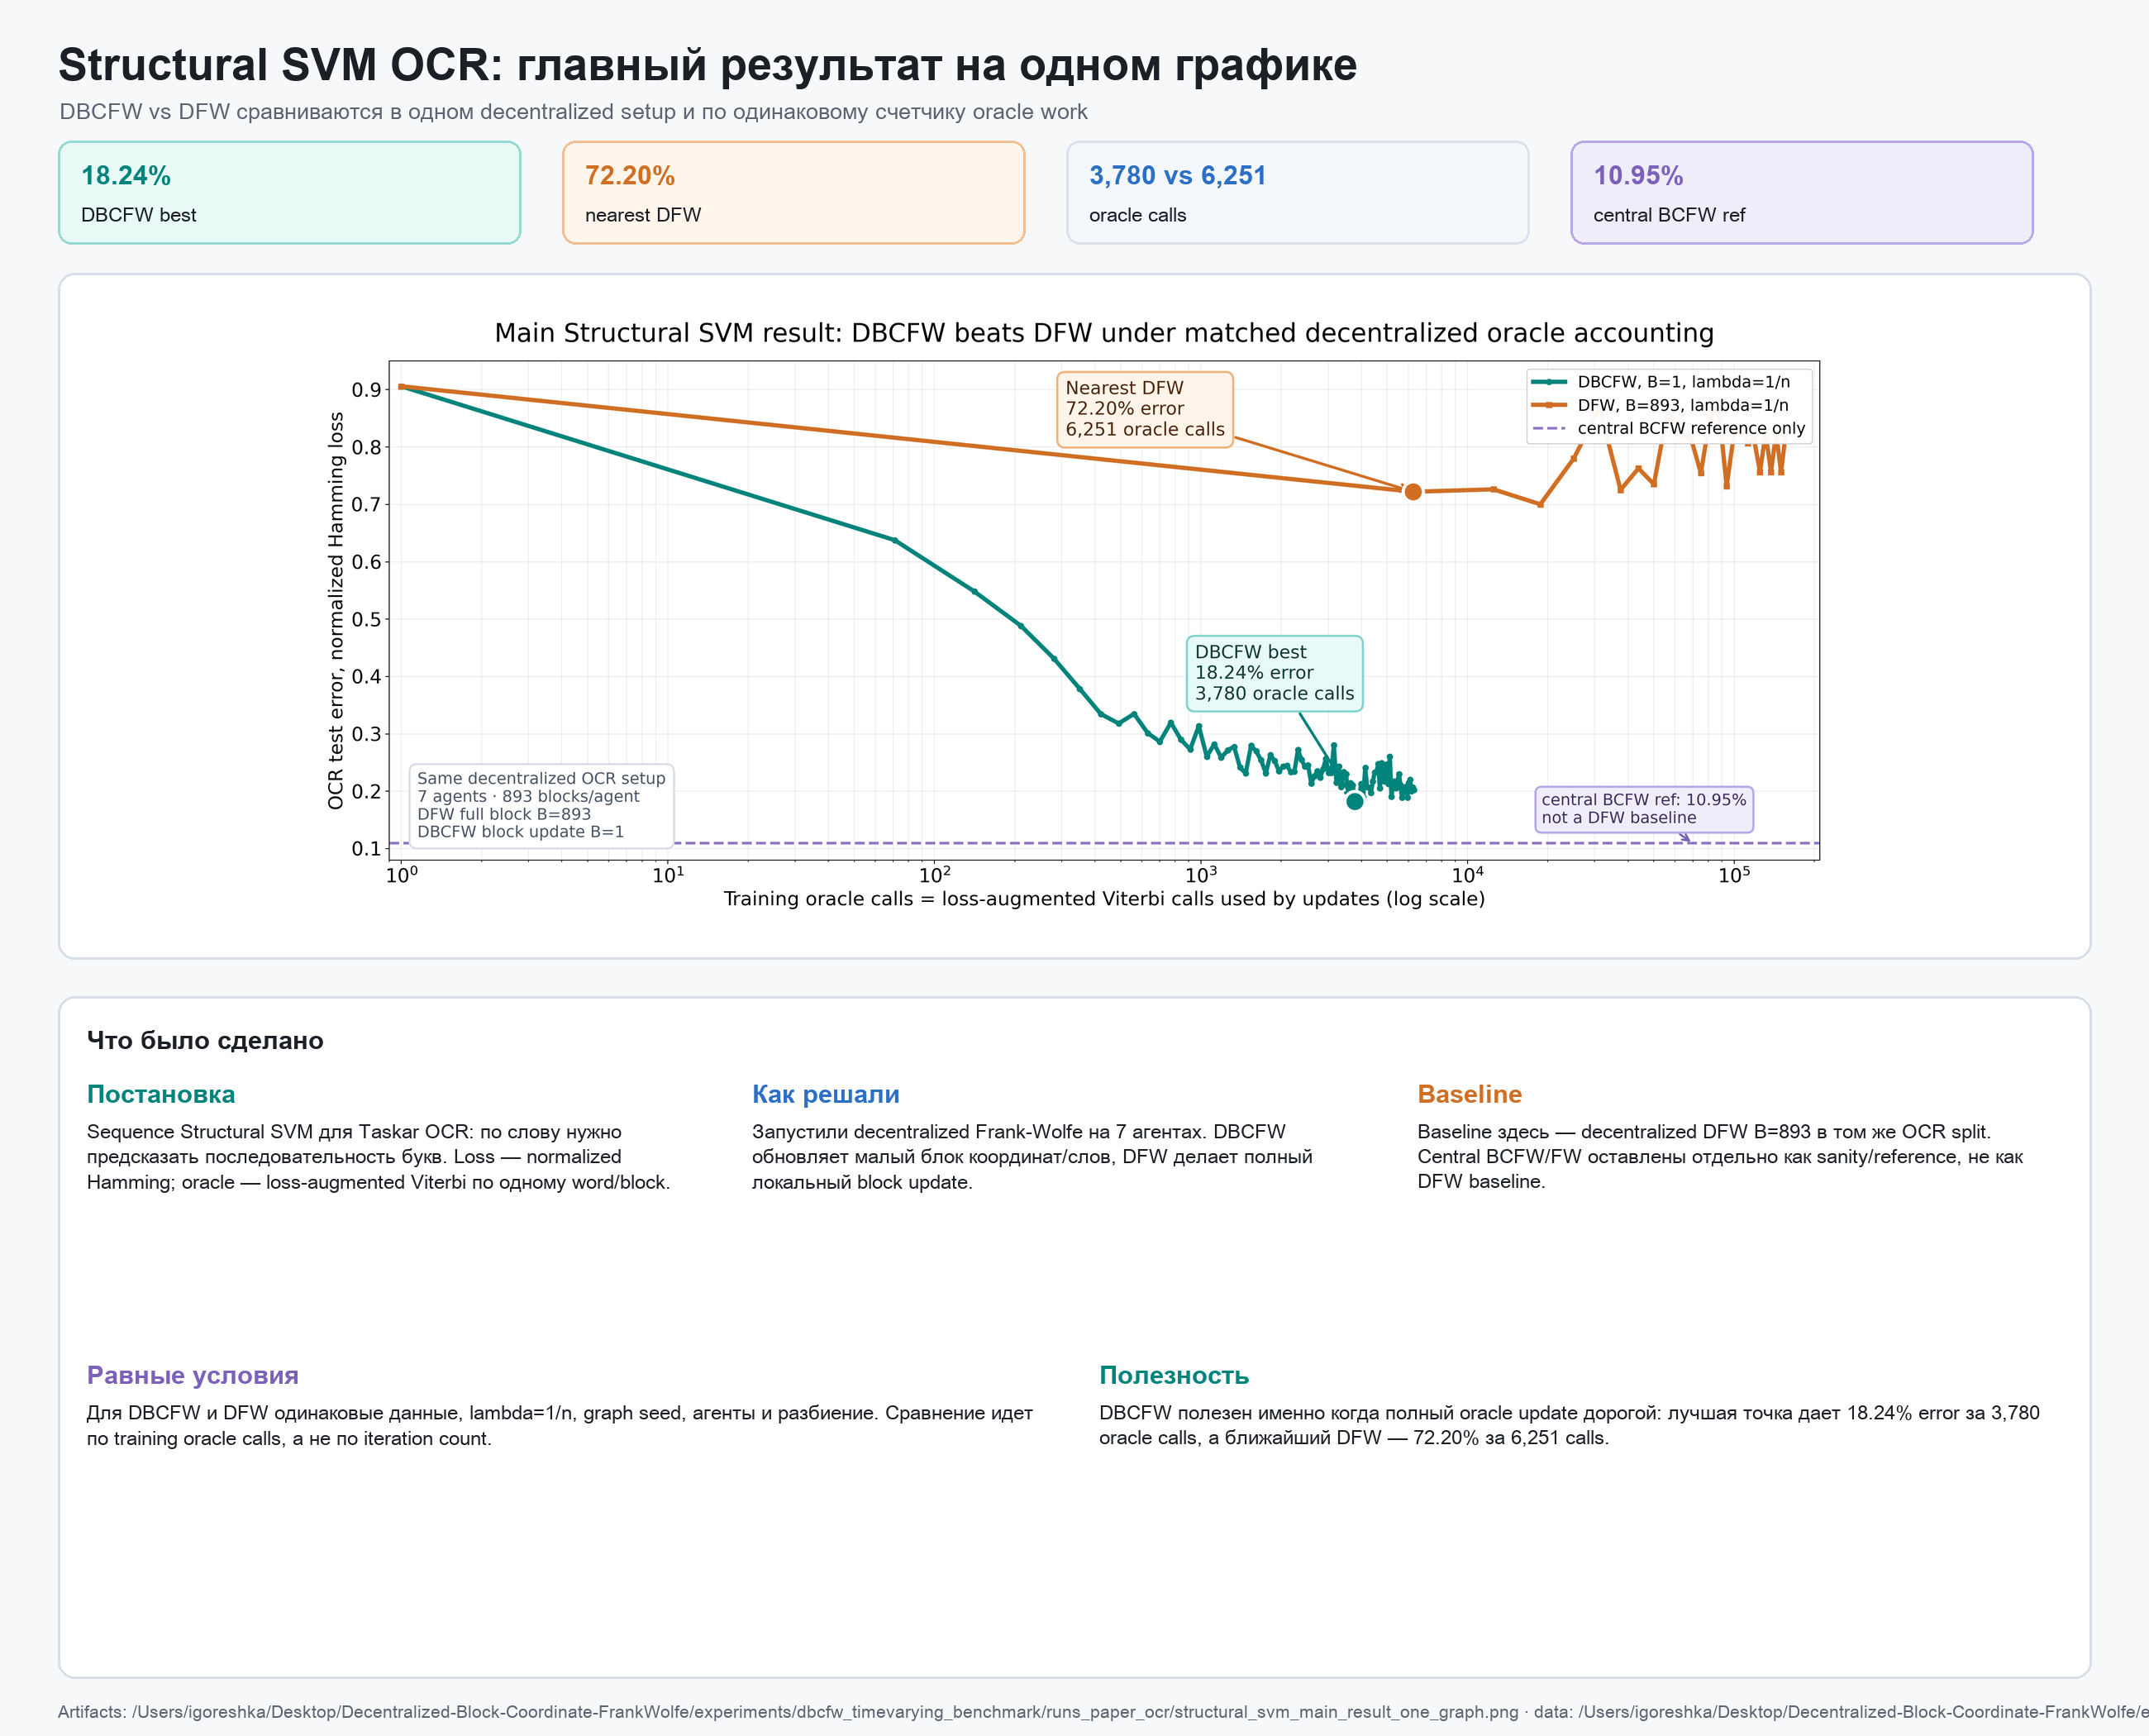
\includegraphics[width=\linewidth]{figures/main_result_one_graph.png}
  \caption{Main fair comparison on Structural SVM OCR. DBCFW and DFW are compared in the same decentralized setup using training oracle calls on the x-axis. Central BCFW is shown only as a reference line.}
  \label{fig:main-result}
\end{figure}

The best fair DBCFW point in the main run is:
\[
  \lambda = 1/n,\quad B=1,\quad \text{iteration}=540,\quad
  \text{training oracle calls}=3780.
\]
At that point, test error is \(18.24\%\). The nearest DFW point for the same \(\lambda\) has 6,251 training oracle calls and \(72.20\%\) test error. Thus, under oracle-work accounting, DBCFW is about
\[
  \frac{72.20}{18.24}\approx 3.96
\]
times lower in test error at the highlighted comparison point.

\begin{table}[htbp]
\centering
\caption{Decentralized DBCFW vs DFW matched by nearest training-oracle budget. Lower test error is better.}
\resizebox{\linewidth}{!}{%
\begin{tabular}{llrrrrrrrrr}
\toprule
\(\lambda\) & \(B\) & DBCFW iter & DBCFW oracle & DBCFW test & DBCFW gap & DFW iter & DFW oracle & DFW test & DFW gap & ratio \\
\midrule
0.01  & 1  & 740 & 5180  & 19.11\% & 0.556 & 1  & 6251  & 72.20\% & 2      & 3.78x \\
0.01  & 10 & 55  & 3850  & 27.81\% & 8.31  & 1  & 6251  & 72.20\% & 2      & 2.60x \\
0.01  & 89 & 95  & 59185 & 58.92\% & 371   & 9  & 56259 & 84.99\% & 263    & 1.44x \\
0.001 & 1  & 580 & 4060  & 18.44\% & 0.568 & 1  & 6251  & 72.20\% & 2      & 3.91x \\
0.001 & 10 & 120 & 8400  & 28.31\% & 88.7  & 1  & 6251  & 72.20\% & 2      & 2.55x \\
0.001 & 89 & 155 & 96565 & 56.03\% & \(4.65{\times}10^3\) & 15 & 93765 & 68.21\% & \(2.63{\times}10^4\) & 1.22x \\
1/n   & 1  & 540 & 3780  & 18.24\% & 0.583 & 1  & 6251  & 72.20\% & 2      & 3.96x \\
1/n   & 10 & 75  & 5250  & 26.65\% & 546   & 1  & 6251  & 72.20\% & 2      & 2.71x \\
1/n   & 89 & 50  & 31150 & 56.86\% & \(3.62{\times}10^4\) & 5 & 31255 & 86.77\% & 30.8 & 1.53x \\
\bottomrule
\end{tabular}}
\label{tab:decentralized}
\end{table}

\section{Central sanity reference}

The central validation reproduces the expected qualitative behavior from the BCFW Structural SVM literature: BCFW is much stronger than full central FW on this OCR task. This validates that the local Structural SVM objective and loss-augmented Viterbi oracle are behaving sensibly. It is not the baseline for the decentralized DFW comparison.

\begin{table}[htbp]
\centering
\caption{Central BCFW vs FW validation. This table is a sanity reference, not a decentralized DFW baseline.}
\begin{tabular}{lrrrrrrr}
\toprule
\(\lambda\) & BCFW best & pass & BCFW final gap & FW best & pass & FW final gap & ratio \\
\midrule
0.01  & 11.72\% & 20 & 0.00404 & 17.38\% & 137 & 0.627 & 1.48x \\
0.001 & 11.09\% & 35 & 0.0684  & 16.97\% & 138 & 0.692 & 1.53x \\
1/n   & 10.95\% & 75 & 0.221   & 17.72\% & 132 & 0.627 & 1.62x \\
\bottomrule
\end{tabular}
\label{tab:central}
\end{table}

\section{Why the comparison is fair}

The comparison is fair in the following restricted sense:
\begin{itemize}
  \item DBCFW and DFW use the same OCR split and same train/test examples.
  \item Both use the same decentralized partition: 7 agents and 893 word blocks per agent.
  \item Both use the same graph model, seed, and regularization value in the highlighted result.
  \item Both are measured by training loss-augmented Viterbi oracle calls, which is the dominant expensive primitive for Structural SVM training.
  \item The DFW baseline is decentralized DFW, not central FW.
\end{itemize}

The comparison is not a claim that DBCFW is universally better under every cost model. DBCFW uses many more communication rounds: the highlighted DBCFW point uses 540 decentralized iterations, while the nearest DFW point uses one full-block iteration. Therefore, the strongest claim supported by this experiment is oracle efficiency: DBCFW is much better when loss-augmented inference is expensive relative to communication.

\section{Why DBCFW wins here}

The main reason is the mismatch between update granularity and oracle cost. A DFW step is a full local block update and costs 6,251 loss-augmented Viterbi oracle calls. In the same oracle budget, DBCFW with \(B=1\) can perform hundreds of small, targeted block updates. In this OCR run, DBCFW reaches a useful model before DFW completes even one full expensive update.

The second reason is numerical stability in the current decentralized implementation. In the logged run for \(\lambda=1/n\), the highlighted DBCFW point has test error \(18.24\%\), objective gap \(0.583\), and consensus error \(0.283\). DFW at later iterations develops very large objective gaps and consensus errors. This suggests that full-block decentralized updates need more careful scaling, line-search, or state averaging before they become a competitive baseline on this Structural SVM task.

\section{Conclusion}

The experiment supports the following conclusion:

\begin{quote}
For decentralized Structural SVM OCR training, block-coordinate decentralized Frank-Wolfe is substantially more oracle-efficient than full-block decentralized Frank-Wolfe. The best DBCFW point reaches \(18.24\%\) test error using 3,780 training oracle calls, while the nearest DFW point reaches only \(72.20\%\) test error using 6,251 calls. Central BCFW remains better at \(10.95\%\), so the decentralized method is useful but not yet at central paper-quality performance.
\end{quote}

\bibliographystyle{plainnat}
\bibliography{references}

\end{document}
